\documentclass{article}

% if you need to pass options to natbib, use, e.g.:
% \PassOptionsToPackage{numbers, compress}{natbib}
% before loading nips_2016
%
% to avoid loading the natbib package, add option nonatbib:
% \usepackage[nonatbib]{nips_2016}

\PassOptionsToPackage{numbers,sort&compress}{natbib}
\usepackage[final]{nips_2016} % produce camera-ready copy

\usepackage[utf8]{inputenc} % allow utf-8 input
\usepackage[T1]{fontenc}    % use 8-bit T1 fonts
\usepackage{hyperref}       % hyperlinks
\usepackage{url}            % simple URL typesetting
\usepackage{booktabs}       % professional-quality tables
\usepackage{amsfonts}       % blackboard math symbols
\usepackage{nicefrac}       % compact symbols for 1/2, etc.
\usepackage{microtype}      % microtypography
\usepackage{subcaption}
\captionsetup{compatibility=false}
\usepackage{graphicx}

\title{Predicting Song Popularity Based on Top 200 Spotify Ranking}

% The \author macro works with any number of authors. There are two
% commands used to separate the names and addresses of multiple
% authors: \And and \AND.
%
% Using \And between authors leaves it to LaTeX to determine where to
% break the lines. Using \AND forces a line break at that point. So,
% if LaTeX puts 3 of 4 authors names on the first line, and the last
% on the second line, try using \AND instead of \And before the third
% author name.

\author{
  S2194678\\
  %% examples of more authors
  \And
  S2015320\\
 \And
  S2759284\\
  \And
  S2710401\\
}

\begin{document}

\maketitle

\begin{abstract}

This study investigates the factors contributing to song popularity. It focuses on the correlation between musical features (numerical) and rankings in Spotify's Top 200 daily chart. Study explores the role of an artist in the popularity of the song. The dataset, comprising over 651,000 entries and 20 features such as acousticness, energy, and danceability, was preprocessed to standardise numerical values, encode cyclic patterns, and transform textual data using Word2Vec. Principal Component Analysis (PCA) was applied for dimensionality reduction and feature importance evaluation. Both unsupervised and supervised learning methods were used. Methods used consist of clustering and classification models such as Decision Trees, Random Forest, and Gradient Boosting, to predict song rankings. Key findings highlight seasonal patterns in musical preferences, with features such as energy and danceability varying during festive periods. While supervised models demonstrated potential, limitations arose due to omitted external factors like marketing, regional preferences and others. Future research directions include incorporating lyrical analysis, genre classification, and exploring semi-supervised learning methods for enhanced prediction accuracy. The findings underscore the complexity of modelling song popularity and the need for more comprehensive approaches to achieve robust predictions.

\end{abstract}

\section{Introduction}

Spotify is one of the many online platforms that gives users access to millions of songs, albums, and original podcasts. It functions as a digital music service for artists to promote their work \cite{Pedroche2020} . To optimise the user experience, Spotify uses the Natural Language Processing algorithms, also referred to as classification models. By identifying certain keywords, these algorithms provide suggestions for suitable artists, albums, and playlists with the aid of artificial intelligence (AI). \cite{Bjorklund2022} The team at Spotify uses Machine Learning (ML) to detect correlations between new tracks and albums to automatically allocate them to the correct artist’s page. Spotify has multiple ML models that cover a vast range of catalogues that aid it in performing various tasks like categorisation and recommendations. \cite{SpotifyAnnotations2024} 

Spotify compiles a Top 200 daily top rankings, containing the most listened-to songs on a daily basis. There are several publications that have previously explored the ranking list, looking at correlations within data by employing various machine learning tasks. \cite{Luo2018} This dataset was provided by the teaching staff of the course, but a version of it could have been downloaded from Kaggle.com, a data science platform \cite{kaggle2024top200}. The list contains several features like acousticness, danceability, energy, loudness, speechiness, instrumentalness, and valence, alongside data regarding the title, the artist, the country and the continent, associated with each artist.

In this study, the focus is to investigate the correlation between the features and the ranking of the songs on the list. It is crucial to narrow down the characteristics promoting the popularity of songs, to improve the understanding of their role in the ranking. The aim is to implement various unsupervised and supervised learning methods to compare the accuracy of the models and suggest the optimal approach to employ for song rank prediction.


\section{Data Analysis}
The original dataset includes 651936 rows of daily data entries for 7457 unique songs. These entries comprise a 651936 x 20 matrix, which includes a daily top 200 song ranking. However, some songs were present multiple times in a day differing by only one column - the artist. These entries are treated as collaborators.

\subsection{Data Preprocessing and Dimensionality Reduction}

The dataset consisted of no null values. Hence, it could be used for further processing as it is considered a clean/complete dataset. Each row of the dataset consisted of the title of the song, the artists involved, the nationality and continent of these artists, and other feature metrics of the song - danceability, speechiness, acousticness, loudness, etc. Each song also had a 'Points' column that was calculated by the peak rank of the song. Due to the direct correlation between points and rank, any points field was dropped. Some of these characteristic song features such as loudness, energy etc were reported in different scales and had to be normalised. The default \textit{StandardScaler()} method of SciKitLearn was used to standardise these fields. Upon standardising, all the values were represented with a mean of 0 and a standard deviation of 1.  The 'Date' field was first converted from type \textit{object} to type \textit{DateTime}. For ease of use, this was further divided into day, month and year with the original date columns dropped due to redundancy. However, that means the future model would not be able to capture cyclic patterns (e.g., January is closer to December than to July). To address this issue, sine and cosine transformations were used to encode day and month. For a cyclic feature \textit{x} with a maximum value \textit{M}:

\[
\text{sin\_encoded} = \sin\left(\frac{2\pi x}{M}\right)
\]
\[
\text{cos\_encoded} = \cos\left(\frac{2\pi x}{M}\right)
\]
This transforms the cyclic feature into two components that represent its position on a circle.

Apart from these numeric columns, there were many features comprised of textual data. These had vital information about the songs and their singers which played a crucial role in the classification model as explained in the later sections. These features were processed using Word2Vec. Gensim was used to implement this. It converted each text value of one feature to a vector in the space, and the positioning of the vectors was based on the words' semantic meanings and proximity to other words. To maintain uniformity, these vectors were also standardised. 

As part of preprocessing, dimensionality reduction was also performed using Principal Component Analysis (PCA). This step plays a crucial role in reducing high-dimensional data into simpler data with fewer features while preserving most of the variance. The aim was to simplify and improve the models' performance by reducing the overfitting and the time required for the training phase. From the result of the elbow plot, the number of principal components was chosen to be 6. 


A new column called 'Ranking' was created based on the 'Rank' of each song. This column divided the database into 4 basic bins such that songs with ranks 1 to 20 fall under bin 1. Songs with ranks 21 to 50 are placed under bin 2, with ranks from 51 to 100 in bin 3 and finally all songs with ranks above 100 in bin 4. This feature is a target variable and will not be used in any of the training. The new transformed dataset was now ready for exploratory data analysis. 

Artist was hypothesised to be a good factor in whether a song will become popular. Many people listen to songs based on the artist since they typically release similar types of songs and not song content. To calculate the artist weight we worked out the mean rank of all their song performances and then normalised the data to achieve a weight between 0 and 1.

\subsection{Exploratory Data Analysis}

%<We cant talk about correlation graph here because we have already applied PCA. Because of that. the components will be orthogonal to each other. Hence, apart from the principal diagonal, all other values will be 0.>

Before diving into model creation, the data was analysed to find some meaningful trends. For example, the danceability feature was plotted against the time and it showed that every year during Christmas and New Year times, the average danceability dropped drastically. On plotting the feature energy over time, a similar drop can be seen during the same Christmas and New Year period. This can be observed in Figure \ref{fig:example}. This is most probably due to people playing Christmas carols during these times. 

\begin{figure}%
    \centering
    \subfloat[\centering Danceability vs Time]{{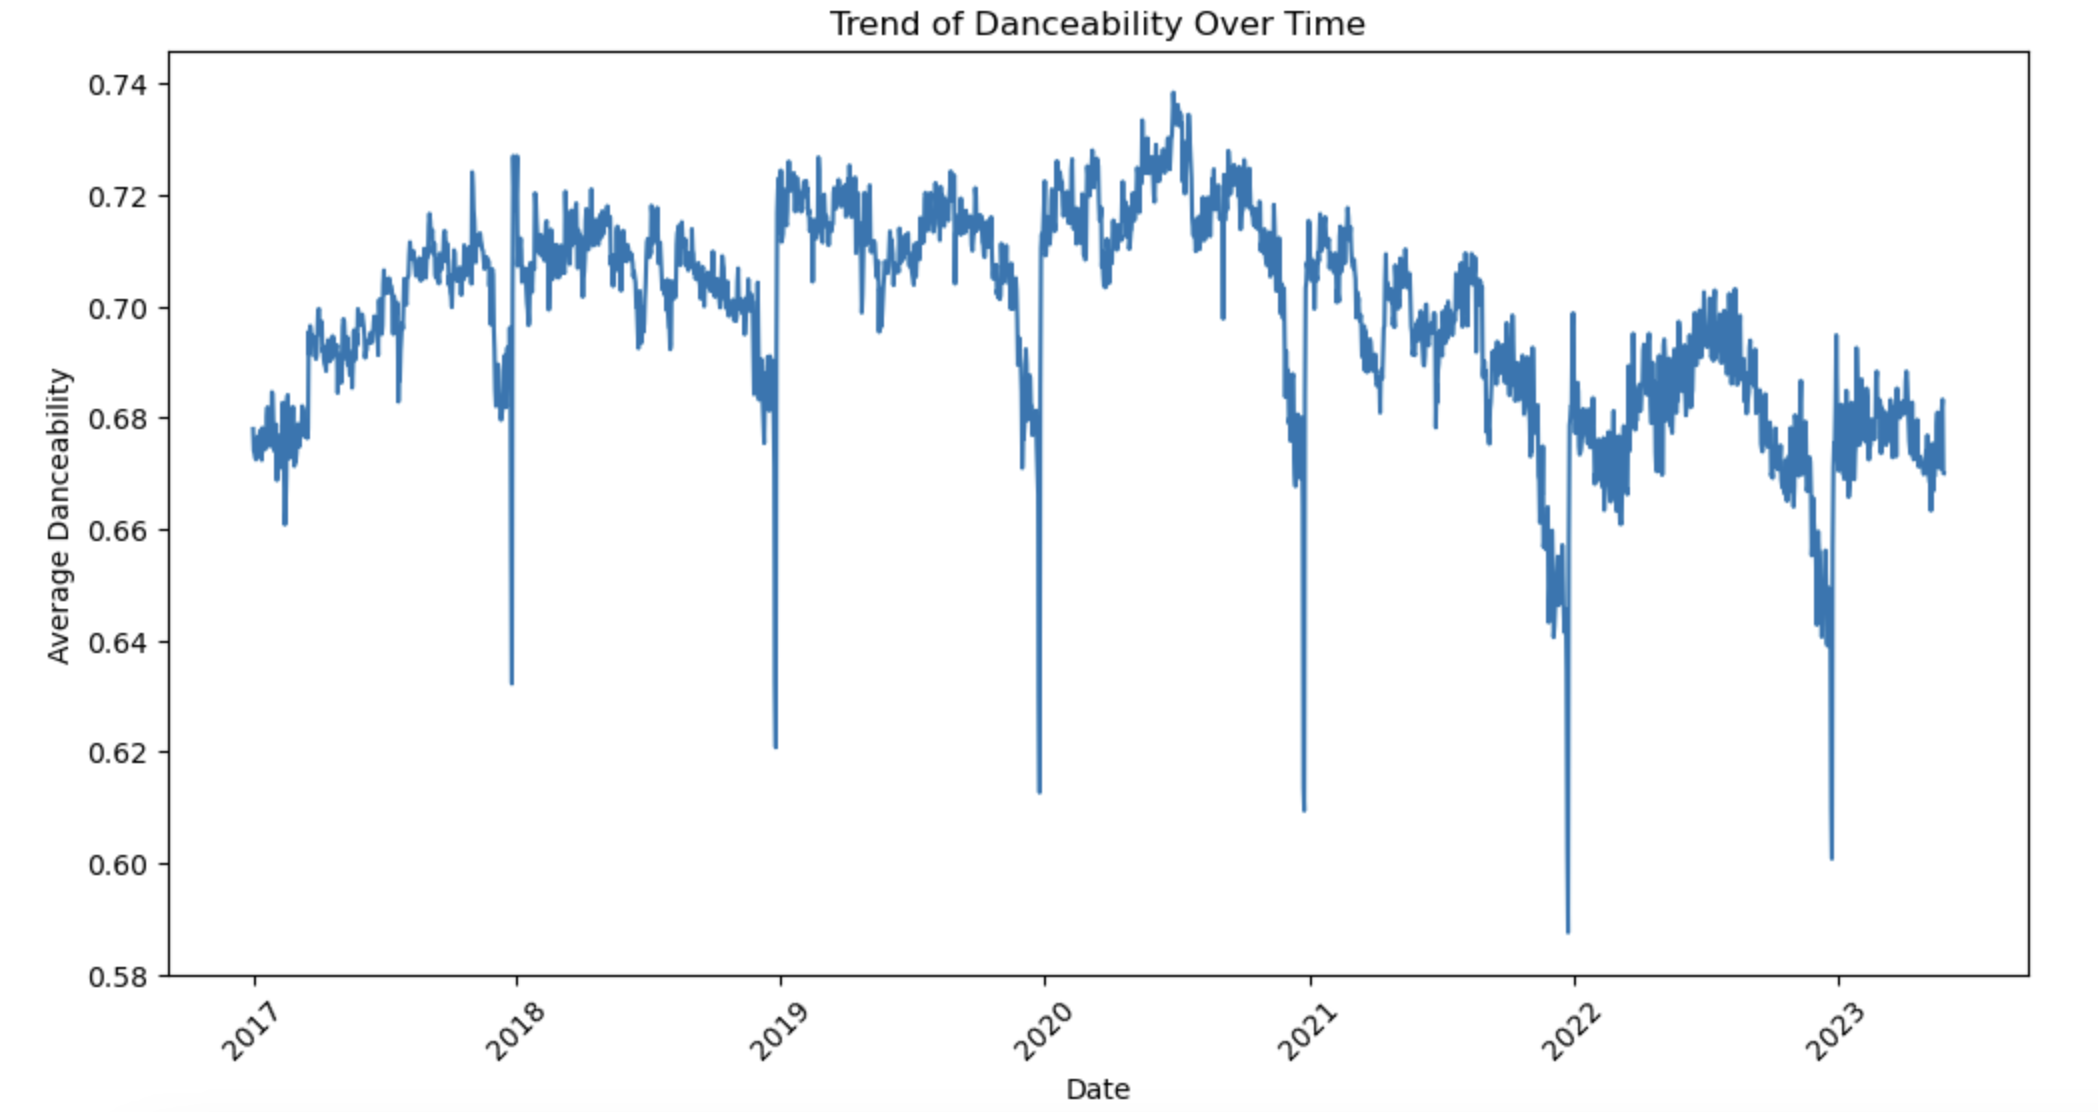
\includegraphics[width=6.5cm]{Danceability.png} \label{1fig} }}%
    \qquad
    \subfloat[\centering Energy vs Time]{{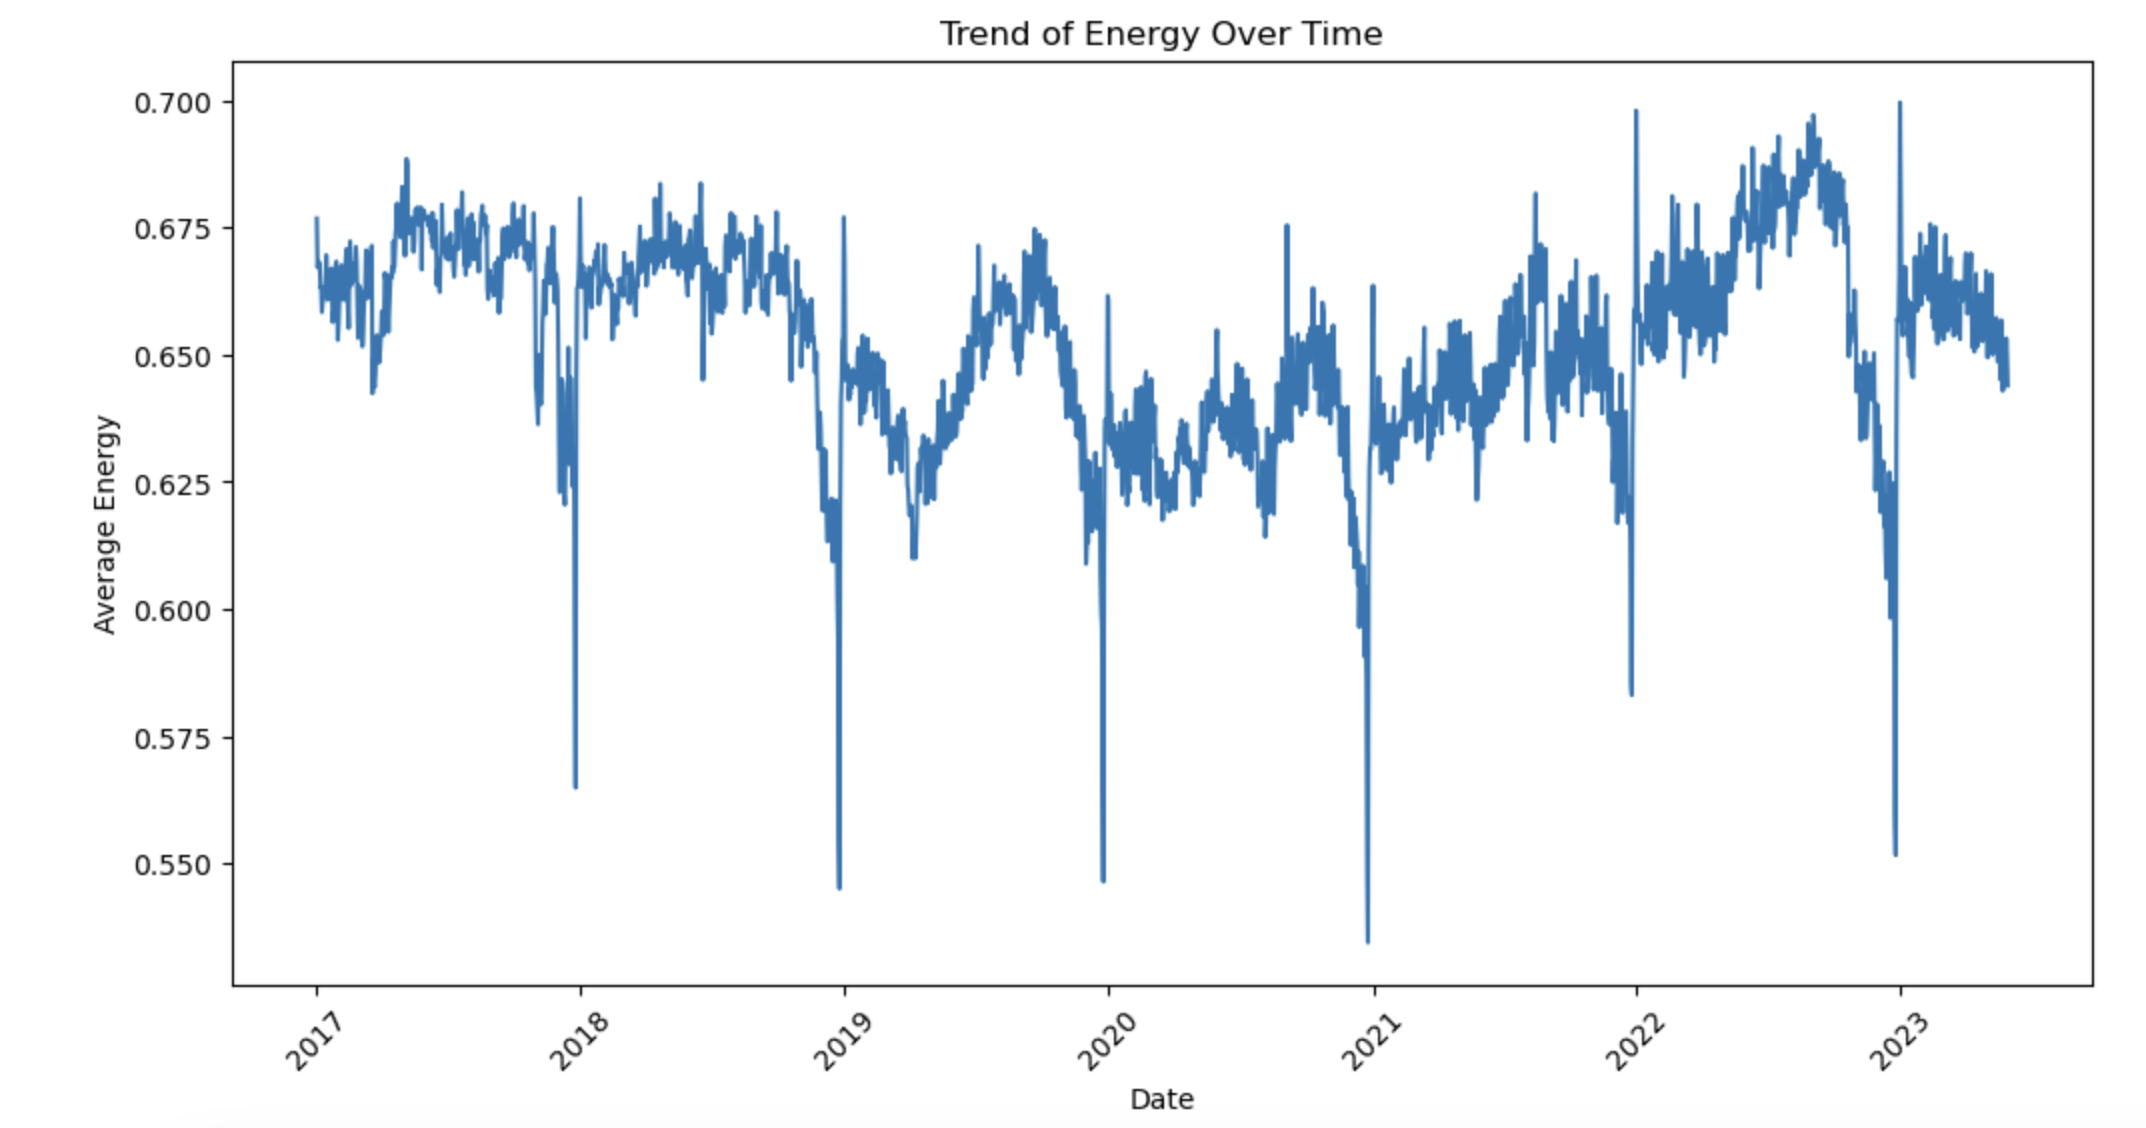
\includegraphics[width=6.5cm]{Energy.png} \label{2fig}}}%
    \caption{Trends of features plotted against time}%
    \label{fig:example}%
\end{figure}



\subsection{Learning Methods}

\subsubsection{PCA}

Initially Principal Component was done just to reduce the dimensionality of the data. Additionally, it was revisited at a later stage to find even more insights about the data. This time PCA was used to determine the most effective parameters. First, an elbow plot was created in order to explain the number of components that were appropriate when regression characteristics of the principal components were assessed. That number of components was used to carry out the transformation of the dataset based on the elbow point. 

To evaluate the importance of each feature, the absolute weights of each feature across all principal components were added together. Cumulative contributions were calculated to form a ranking of the features in which they are arranged according to their extent on the structure of the dataset. This approach made it easier to identify the principal features, thus helping in understanding the critical features of the dataset.

K-Means clustering was then performed using the data which is not high dimensional. The clusters formed are as shown in Figure \ref{fig:clust}, where it was observed that the groups were distinct and the data had structure. The fused PCA increased the level of dimension reduction, cut off unnecessary noise and ensured that the most appropriate features were enhanced, which boosted the quality of the clustering.
\begin{figure}[h]
\centering
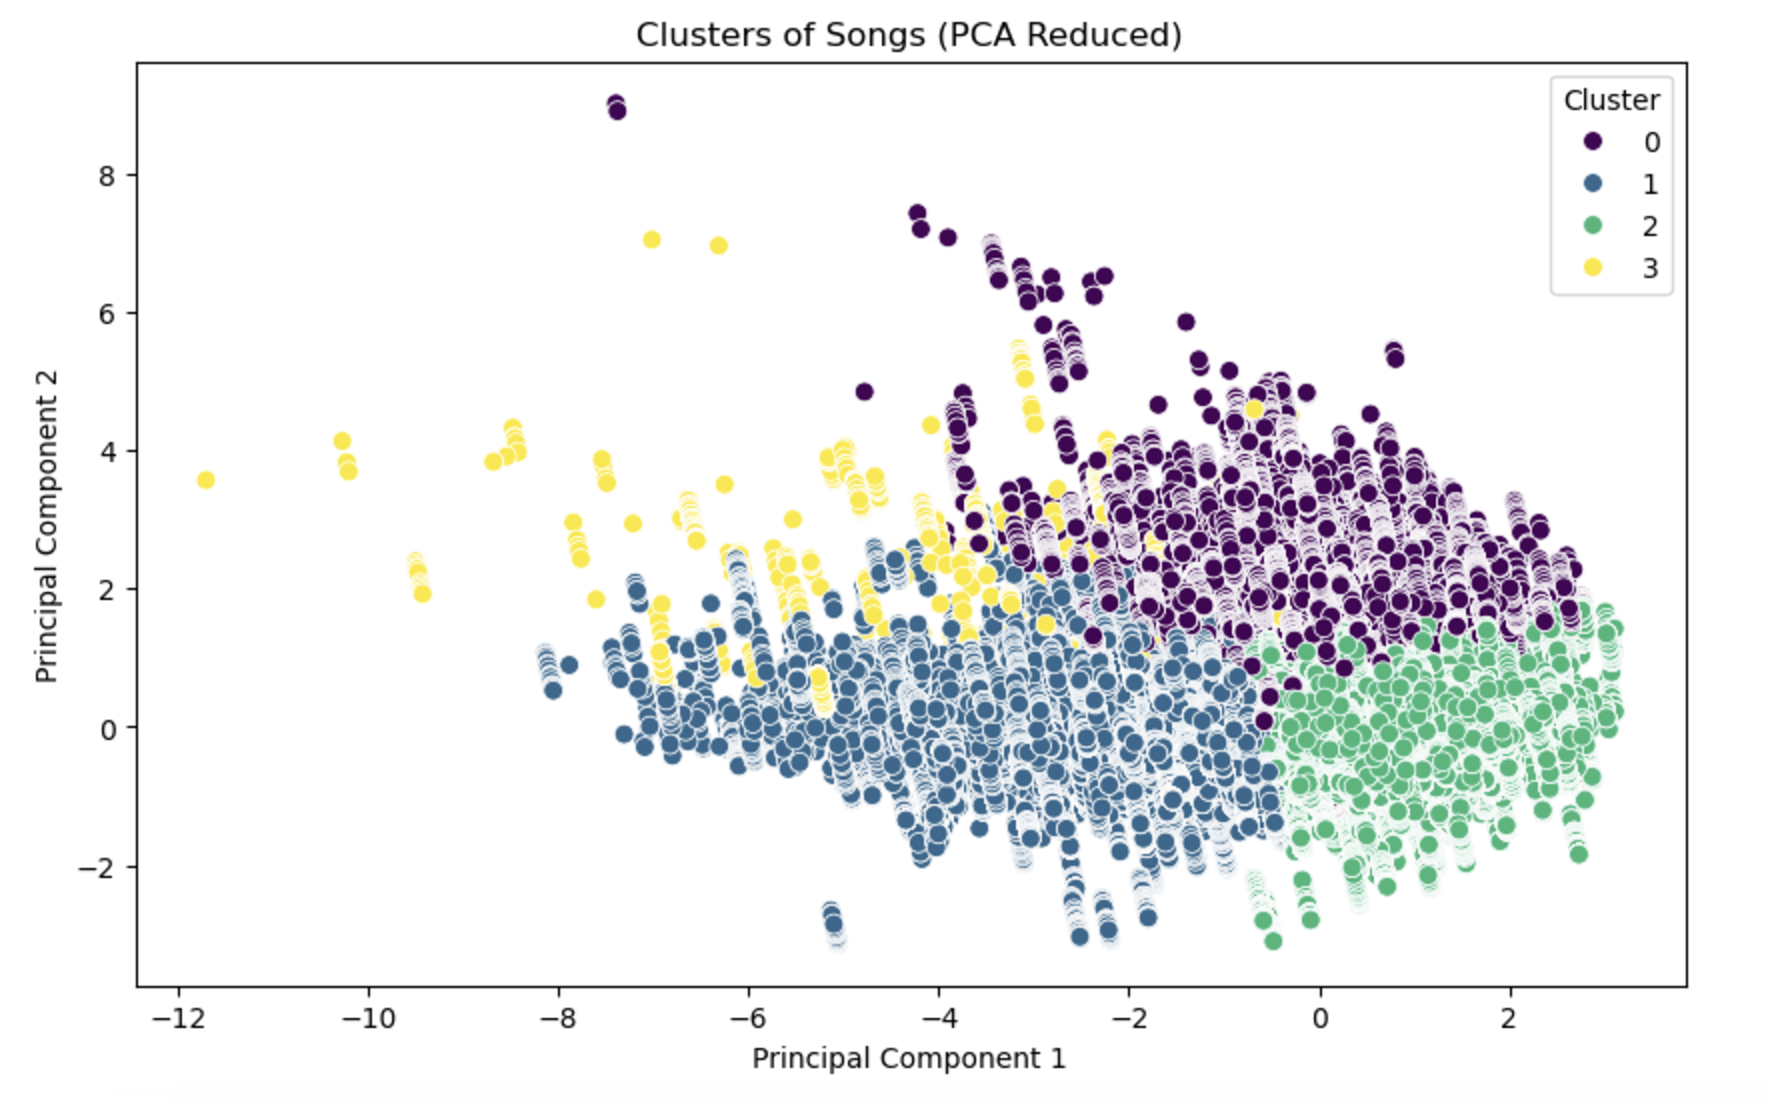
\includegraphics[width=0.7\textwidth]{kmeans.png}
\caption{Clustering after PCA}
\label{fig:clust}
\end{figure}

% \end{itemize}

\subsubsection{Supervised Models}
Supervised learning entails using labelled datasets to train the algorithms. It looks for patterns between inputs and outputs, by mapping inputs to outputs.
\cite{nasteski2017overview} Various different models were used, including Decision Trees, Random Forest, Logistic Regression, Gradient Boosting, KNN, and SVM. 

\textbf{Decision Trees} use a tree-like structure for data classification and are one of the most common classification models due to their versatility and their ability to work with non-numerical data \cite{priyam2013comparative}. \textbf{Random Forest} combines the outcomes from classifiers like Decision Trees, achieving high classification accuracy, when handling large datasets \cite{parmar2019review}. \textbf{Logistic Regression} is based on the mathematical function, the purpose of which is predicting the binary outcome, based on a group of independent variables. That is achieved by quantifying each variable's contribution. Logistic Regression is usually considered for initial screening, as it overfits on high dimensional data. \cite{stoltzfus2011logistic}  \textbf{Gradient Boosting} was chosen for its performance with class imbalance percentages and due to it resulting in improved speed of predictive models \cite{bentejac2021comparative}. K-nearest neighbours \textbf{(KNN)} predicts the classification of the new unlabeled data, based on the labeled training data. It is based on the local minimum of the target function and can work with complex decision boundaries. \cite{Hamilton2020} Support vector machine \textbf{(SVM)}, the final model considered, creates a hyperplane, which enhances the margin between the data points on the n-plane. It has been classified as one of the most robust classification tools, cited in many score prediction papers \cite{Yee2022}.

To predict the song's popularity, the data was split into training and testing datasets  (\( 80\% \) and \( 20\% \) respectively).

\section{Results}
Six different models - Random Forest, Logistic Regression, Support Vector Machine, K-Nearest Neighbor, Gradient Boosting and Decision Tree - were chosen to test. All of the tests were performed on common code testing multiple models in one go. Accuracy, precision, recall as well as F1 scores of each of these models were obtained to determine which of these proved to be the best.

The results aim to explore and predict the rank which has been separated into 4 distinct bins. Top 20, 21 - 50, 51 - 100, 101 - 200. This ensures the models give a higher accuracy as predicting exact ranking is still out of reach. 

Table 1 shows the results given when the model is ran on raw numerical features excluding artists. The results show that numerical data alone such as danceability, loudness etc., cannot predict the song's rank based on them alone. The highest achieved result is 40\% using the Random Forest and Logistic Regression models.


 %I will go back and remove we tense
 
Table 2 shows the result when the artist weight factor is used which was calculated before. This influences the result showing that more popular artists are more likely to score higher. The highest achieved result shows 50\% classification accuracy. This is approximately 5 - 10\% for each model analysed further highlighting the importance of the feature.

Using the above knowledge the model was tested on PCA data including the artist weight factor to see how this affected our results. A plot describing the results is shown in Figure \ref{res}. Logistic Regression and Support Vector Machine proved to be the two highest in accuracy at 96.58\% and 96.71\% respectively. 

As mentioned in section 2.1, the target variable is the 'Ranking' column. Predicting the exact rank of a song based on the features and details given is something that this model is incapable of. Instead, the top model tried to predict the bin in which the song belongs. 
\begin{figure}[h]
\centering
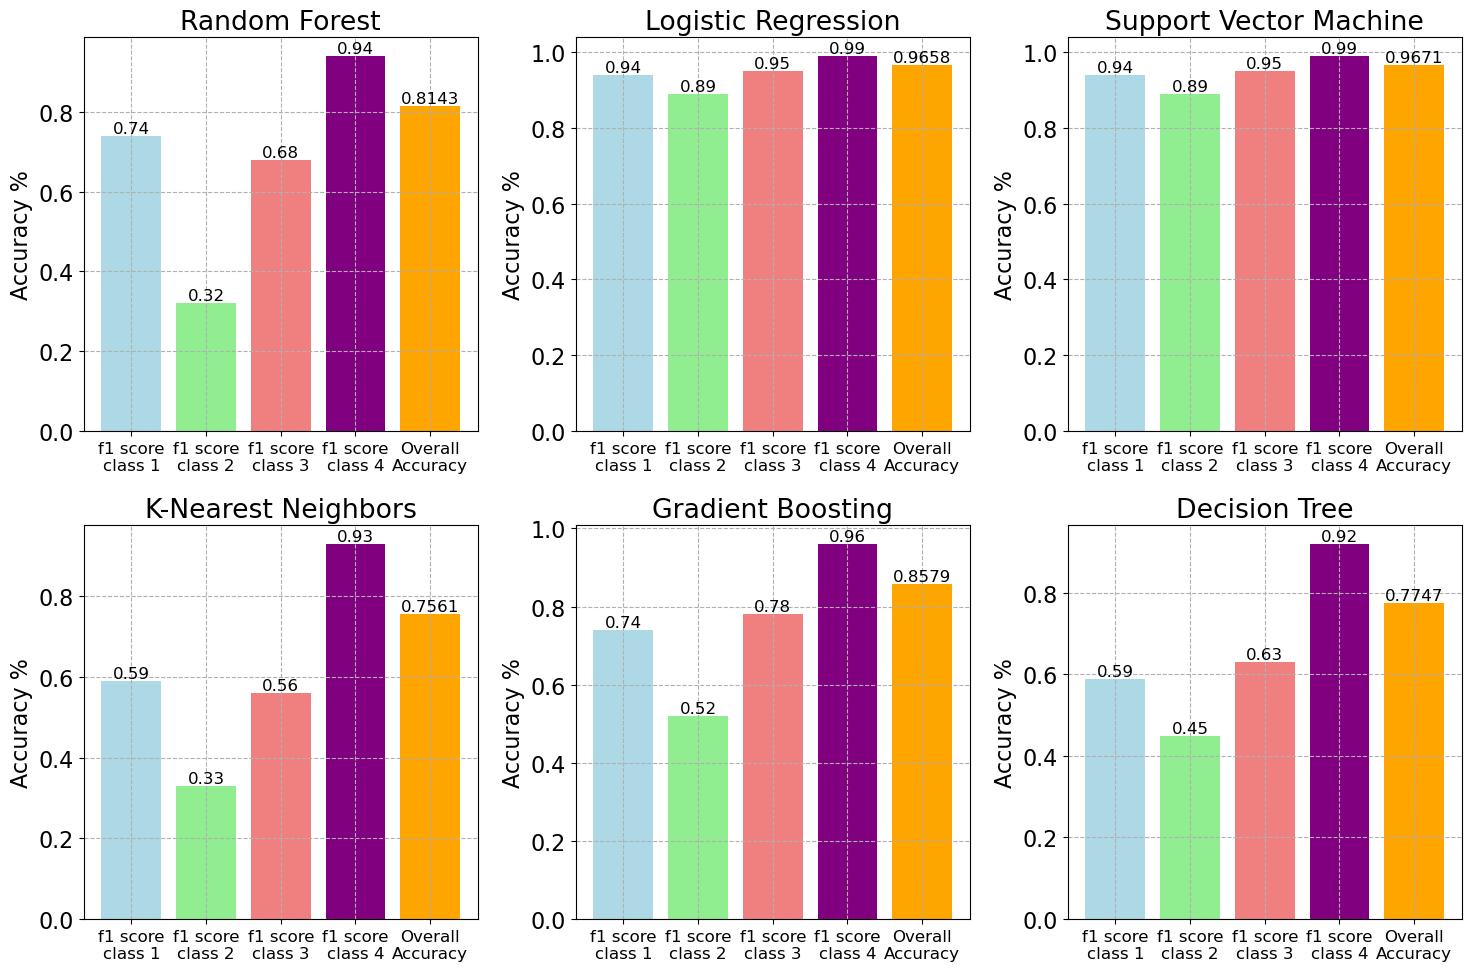
\includegraphics[width=0.99\textwidth]{result.png}

\caption{Comparison of model performance}
\label{res}
\end{figure}


\begin{table}[h]
\centering
\begin{tabular}{|l|c|c|c|c|c|}
\hline
Model & Accuracy & F1-Score (1) & F1-Score (2) & F1-Score (3) & F1-Score (4) \\
\hline
Random Forest & 0.397 & 0.010 & 0.020 & 0.020 & 0.570 \\
Logistic Regression & 0.397 & 0.000 & 0.000 & 0.000 & 0.570 \\
K-Nearest Neighbors & 0.284 & 0.200 & 0.200 & 0.280 & 0.360 \\
Gradient Boosting & 0.391 & 0.020 & 0.070 & 0.090 & 0.560 \\
Support Vector Machine & 0.391 & 0.020 & 0.030 & 0.020 & 0.560 \\
Decision Tree & 0.371 & 0.060 & 0.070 & 0.130 & 0.540 \\
\hline
\end{tabular}
\caption{Model Evaluation Results - Excluding Artist}
\label{table:results}
\end{table}


\begin{table}[h]
\centering
\begin{tabular}{|l|c|c|c|c|c|}
\hline
Model & Accuracy & F1-Score (1) & F1-Score (2) & F1-Score (3) & F1-Score (4) \\
\hline
Random Forest & 0.475 & 0.510 & 0.080 & 0.240 & 0.630 \\
Logistic Regression & 0.461 & 0.490 & 0.010 & 0.210 & 0.630 \\
K-Nearest Neighbors & 0.364 & 0.360 & 0.200 & 0.280 & 0.500 \\
Gradient Boosting & 0.454 & 0.520 & 0.160 & 0.280 & 0.590 \\
Support Vector Machine & 0.438 & 0.450 & 0.190 & 0.280 & 0.590 \\
Decision Tree & 0.442 & 0.500 & 0.230 & 0.330 & 0.570 \\
\hline
\end{tabular}
\caption{Model Evaluation Results - Including Artist}
\label{table:results}
\end{table}



\subsection{Limitations}

The study has several limitations which could be used as motivation and areas of improvement in the future to further expand on the topic. The study only considers first-listed artists on collaborative tracks completely disregarding the influence of co-artists. This commission skews a minority of the results, especially for tracks that collaborations make the song popular.

Another limitation of the study is modelling assumptions. The supervised learning models assume that the relationship between features and rank categories is consistent across all songs, which may not hold true for niche genres or outlier cases. Additionally, some models (e.g., Logistic Regression) assume linear relationships between features and outputs, which might oversimplify the complex dynamics of song popularity. 

Another limitation of the study is that global rankings neglect regional differences in music preferences. Songs popular in specific regions or cultural contexts may exhibit distinct characteristics not reflected in the global dataset. The study does not account for external influences, such as marketing, social media trends, or viral phenomena, which often drive transient or sustained chart success. Building upon trends we neglect to consider trends. As analysed before music preference changes per season with the biggest change being during Christmas.  

Finally, the study analyses a limited set of features, excluding important factors such as genre, lyrical semantics, country-specific popularity, and other relevant attributes.

\section{Conclusions}

 Our results show that using support vector machine model we can achieve 96.7\% accuracy. The results show when artist weighting is considered then our classification result increases by [5 - 10\%]. Further, using normalised and processed data our rank prediction scores increase significantly giving us a prediction model which is no longer guessing but predicting. Our results show that predicting rank using data values such as danceability, energy, and loudness is not meaningful and an improved model should include and categorise our songs more on semantic and external details, such as genre, social media popularity and radio popularity. For example, currently due to not considering genre a rap song might have been number one at some point, but our model might disagree as it uses the mean features, there was no way of determining it without additional data. The difference in the numerical features of the songs extends which makes our models less precise.

Our findings additionally demonstrate that a song's rank has a great effect on chart lifetime. In most cases a song that is ranked one will stay on the top 200 list way longer than a song that is ranked 100. Nonetheless, there were seasonal outliers that would have never reached the top 20 and would not have outperformed a range of songs.

The finds show and demonstrate that a simple analysis of musical features is not coherent enough to give a detailed rank/popularity explanation. For further and more meaningfull understanding, implementing addition semantic understanding features and well as geographical data will prove to create a more precise model which may not require bin rankings.

\subsection{Future Directions}

Expanding this project in the future presents numerous opportunities for improvement. In addition to a song's melody, its lyrics play a crucial role in defining its appeal. Songs with lyrics that align closely with a specific genre often contribute significantly to the overall rank achieved. In the provided dataset, Spotify does not label the genre, however, previous researchers have utilised Discogs, a music database website, via its API, and merged the datasets \cite{Luo2018}. This exploration paired with textual analysis could enhance the predictive power of used models. This area of investigation could also explain the rise of lesser-known artists and identify features that contribute to their success.

Another promising avenue for future research is the analysis of social media promotions and marketing strategies to discover trends in strong growth. This could involve comparing temporary popularity spikes (where a song briefly charts and has a rapid decline) against sustained popularity gains (where a song consistently ranks high due to its features rather than trends). Such analysis could provide a deeper understanding of external influences.

With the increasing interest in deep learning algorithms, employing a semi-supervised learning (SSL) algorithm could further advance this project. It is predicted that SSL methods of consistency regularisation and generative models could soon reach the accuracy levels of supervised models. Adding SSL to the project could improve the overall performance and add more depth to the results. It has been shown that SSL learns from noisy labels, filters them out, and utilises noisy examples as part of the training, hence optimising the work procedure, by reducing the noise significance. There are not a lot of publications for the Top 200 Spotify ranking with SSL, so adding it could enhance the final prediction accuracy. \cite{Ouali2020}

\pagebreak

\bibliography{refs.bib}
\bibliographystyle{plain}

\newpage
\section{Member Contribution}


\subsection{S2194678}
Student performed background research into previous work around the topic, which allowed them to gain a deeper understanding of the models being used. They contributed to Exploration of data, future directions, limitations, conclusion and results. They cleaned and built up supervised models from the database given along with the code and visualisations for the report and assisted writing multiple of the sections. 

\subsection{S2015320}
Student performed background research for the topic, which aided them in completing the introduction and learning methods of the report. They contributed to the future directions and the data preprocessing sections. In the practical side of the project they worked on the various supervised learning models, alongside dataset cleaning, which were both later optimised to be included in the report. 

\subsection{S2710401}
Student performed background research to understand more about the data, problems, and possible solutions that can be developed in this project. Worked on pre-processing the data which included standardization of numerical columns, converting textual features to vectors etc. Also worked on the unsupervised side of the project involving PCA and KMeans. Lastly helped plot some figures and write the report. 

\subsection{S2759284}
Student helped in the initial Exploratory Data Analysis. 

\section{Use of Generative AI}

No generative AI was used during given project.

\end{document}

%%% Local Variables:
%%% mode: latex
%%% TeX-master: t
%%% End:
